% Options for packages loaded elsewhere
\PassOptionsToPackage{unicode}{hyperref}
\PassOptionsToPackage{hyphens}{url}
\PassOptionsToPackage{dvipsnames,svgnames,x11names}{xcolor}
%
\documentclass[
]{apa7}

\usepackage{amsmath,amssymb}
\usepackage{iftex}
\ifPDFTeX
  \usepackage[T1]{fontenc}
  \usepackage[utf8]{inputenc}
  \usepackage{textcomp} % provide euro and other symbols
\else % if luatex or xetex
  \usepackage{unicode-math}
  \defaultfontfeatures{Scale=MatchLowercase}
  \defaultfontfeatures[\rmfamily]{Ligatures=TeX,Scale=1}
\fi
\usepackage{lmodern}
\ifPDFTeX\else  
    % xetex/luatex font selection
\fi
% Use upquote if available, for straight quotes in verbatim environments
\IfFileExists{upquote.sty}{\usepackage{upquote}}{}
\IfFileExists{microtype.sty}{% use microtype if available
  \usepackage[]{microtype}
  \UseMicrotypeSet[protrusion]{basicmath} % disable protrusion for tt fonts
}{}
\makeatletter
\@ifundefined{KOMAClassName}{% if non-KOMA class
  \IfFileExists{parskip.sty}{%
    \usepackage{parskip}
  }{% else
    \setlength{\parindent}{0pt}
    \setlength{\parskip}{6pt plus 2pt minus 1pt}}
}{% if KOMA class
  \KOMAoptions{parskip=half}}
\makeatother
\usepackage{xcolor}
\setlength{\emergencystretch}{3em} % prevent overfull lines
\setcounter{secnumdepth}{-\maxdimen} % remove section numbering
% Make \paragraph and \subparagraph free-standing
\ifx\paragraph\undefined\else
  \let\oldparagraph\paragraph
  \renewcommand{\paragraph}[1]{\oldparagraph{#1}\mbox{}}
\fi
\ifx\subparagraph\undefined\else
  \let\oldsubparagraph\subparagraph
  \renewcommand{\subparagraph}[1]{\oldsubparagraph{#1}\mbox{}}
\fi

\usepackage{color}
\usepackage{fancyvrb}
\newcommand{\VerbBar}{|}
\newcommand{\VERB}{\Verb[commandchars=\\\{\}]}
\DefineVerbatimEnvironment{Highlighting}{Verbatim}{commandchars=\\\{\}}
% Add ',fontsize=\small' for more characters per line
\usepackage{framed}
\definecolor{shadecolor}{RGB}{241,243,245}
\newenvironment{Shaded}{\begin{snugshade}}{\end{snugshade}}
\newcommand{\AlertTok}[1]{\textcolor[rgb]{0.68,0.00,0.00}{#1}}
\newcommand{\AnnotationTok}[1]{\textcolor[rgb]{0.37,0.37,0.37}{#1}}
\newcommand{\AttributeTok}[1]{\textcolor[rgb]{0.40,0.45,0.13}{#1}}
\newcommand{\BaseNTok}[1]{\textcolor[rgb]{0.68,0.00,0.00}{#1}}
\newcommand{\BuiltInTok}[1]{\textcolor[rgb]{0.00,0.23,0.31}{#1}}
\newcommand{\CharTok}[1]{\textcolor[rgb]{0.13,0.47,0.30}{#1}}
\newcommand{\CommentTok}[1]{\textcolor[rgb]{0.37,0.37,0.37}{#1}}
\newcommand{\CommentVarTok}[1]{\textcolor[rgb]{0.37,0.37,0.37}{\textit{#1}}}
\newcommand{\ConstantTok}[1]{\textcolor[rgb]{0.56,0.35,0.01}{#1}}
\newcommand{\ControlFlowTok}[1]{\textcolor[rgb]{0.00,0.23,0.31}{#1}}
\newcommand{\DataTypeTok}[1]{\textcolor[rgb]{0.68,0.00,0.00}{#1}}
\newcommand{\DecValTok}[1]{\textcolor[rgb]{0.68,0.00,0.00}{#1}}
\newcommand{\DocumentationTok}[1]{\textcolor[rgb]{0.37,0.37,0.37}{\textit{#1}}}
\newcommand{\ErrorTok}[1]{\textcolor[rgb]{0.68,0.00,0.00}{#1}}
\newcommand{\ExtensionTok}[1]{\textcolor[rgb]{0.00,0.23,0.31}{#1}}
\newcommand{\FloatTok}[1]{\textcolor[rgb]{0.68,0.00,0.00}{#1}}
\newcommand{\FunctionTok}[1]{\textcolor[rgb]{0.28,0.35,0.67}{#1}}
\newcommand{\ImportTok}[1]{\textcolor[rgb]{0.00,0.46,0.62}{#1}}
\newcommand{\InformationTok}[1]{\textcolor[rgb]{0.37,0.37,0.37}{#1}}
\newcommand{\KeywordTok}[1]{\textcolor[rgb]{0.00,0.23,0.31}{#1}}
\newcommand{\NormalTok}[1]{\textcolor[rgb]{0.00,0.23,0.31}{#1}}
\newcommand{\OperatorTok}[1]{\textcolor[rgb]{0.37,0.37,0.37}{#1}}
\newcommand{\OtherTok}[1]{\textcolor[rgb]{0.00,0.23,0.31}{#1}}
\newcommand{\PreprocessorTok}[1]{\textcolor[rgb]{0.68,0.00,0.00}{#1}}
\newcommand{\RegionMarkerTok}[1]{\textcolor[rgb]{0.00,0.23,0.31}{#1}}
\newcommand{\SpecialCharTok}[1]{\textcolor[rgb]{0.37,0.37,0.37}{#1}}
\newcommand{\SpecialStringTok}[1]{\textcolor[rgb]{0.13,0.47,0.30}{#1}}
\newcommand{\StringTok}[1]{\textcolor[rgb]{0.13,0.47,0.30}{#1}}
\newcommand{\VariableTok}[1]{\textcolor[rgb]{0.07,0.07,0.07}{#1}}
\newcommand{\VerbatimStringTok}[1]{\textcolor[rgb]{0.13,0.47,0.30}{#1}}
\newcommand{\WarningTok}[1]{\textcolor[rgb]{0.37,0.37,0.37}{\textit{#1}}}

\providecommand{\tightlist}{%
  \setlength{\itemsep}{0pt}\setlength{\parskip}{0pt}}\usepackage{longtable,booktabs,array}
\usepackage{calc} % for calculating minipage widths
% Correct order of tables after \paragraph or \subparagraph
\usepackage{etoolbox}
\makeatletter
\patchcmd\longtable{\par}{\if@noskipsec\mbox{}\fi\par}{}{}
\makeatother
% Allow footnotes in longtable head/foot
\IfFileExists{footnotehyper.sty}{\usepackage{footnotehyper}}{\usepackage{footnote}}
\makesavenoteenv{longtable}
\usepackage{graphicx}
\makeatletter
\def\maxwidth{\ifdim\Gin@nat@width>\linewidth\linewidth\else\Gin@nat@width\fi}
\def\maxheight{\ifdim\Gin@nat@height>\textheight\textheight\else\Gin@nat@height\fi}
\makeatother
% Scale images if necessary, so that they will not overflow the page
% margins by default, and it is still possible to overwrite the defaults
% using explicit options in \includegraphics[width, height, ...]{}
\setkeys{Gin}{width=\maxwidth,height=\maxheight,keepaspectratio}
% Set default figure placement to htbp
\makeatletter
\def\fps@figure{htbp}
\makeatother

\makeatletter
\makeatother
\makeatletter
\makeatother
\makeatletter
\@ifpackageloaded{caption}{}{\usepackage{caption}}
\AtBeginDocument{%
\ifdefined\contentsname
  \renewcommand*\contentsname{Table of contents}
\else
  \newcommand\contentsname{Table of contents}
\fi
\ifdefined\listfigurename
  \renewcommand*\listfigurename{List of Figures}
\else
  \newcommand\listfigurename{List of Figures}
\fi
\ifdefined\listtablename
  \renewcommand*\listtablename{List of Tables}
\else
  \newcommand\listtablename{List of Tables}
\fi
\ifdefined\figurename
  \renewcommand*\figurename{Figure}
\else
  \newcommand\figurename{Figure}
\fi
\ifdefined\tablename
  \renewcommand*\tablename{Table}
\else
  \newcommand\tablename{Table}
\fi
}
\@ifpackageloaded{float}{}{\usepackage{float}}
\floatstyle{ruled}
\@ifundefined{c@chapter}{\newfloat{codelisting}{h}{lop}}{\newfloat{codelisting}{h}{lop}[chapter]}
\floatname{codelisting}{Listing}
\newcommand*\listoflistings{\listof{codelisting}{List of Listings}}
\makeatother
\makeatletter
\@ifpackageloaded{caption}{}{\usepackage{caption}}
\@ifpackageloaded{subcaption}{}{\usepackage{subcaption}}
\makeatother
\makeatletter
\@ifpackageloaded{tcolorbox}{}{\usepackage[skins,breakable]{tcolorbox}}
\makeatother
\makeatletter
\@ifundefined{shadecolor}{\definecolor{shadecolor}{rgb}{.97, .97, .97}}
\makeatother
\makeatletter
\makeatother
\makeatletter
\makeatother
\ifLuaTeX
  \usepackage{selnolig}  % disable illegal ligatures
\fi
\IfFileExists{bookmark.sty}{\usepackage{bookmark}}{\usepackage{hyperref}}
\IfFileExists{xurl.sty}{\usepackage{xurl}}{} % add URL line breaks if available
\urlstyle{same} % disable monospaced font for URLs
\hypersetup{
  pdftitle={Untitled},
  colorlinks=true,
  linkcolor={blue},
  filecolor={Maroon},
  citecolor={Blue},
  urlcolor={Blue},
  pdfcreator={LaTeX via pandoc}}

\title{Untitled}
\author{}
\date{}

\begin{document}
\maketitle
\ifdefined\Shaded\renewenvironment{Shaded}{\begin{tcolorbox}[interior hidden, boxrule=0pt, borderline west={3pt}{0pt}{shadecolor}, enhanced, breakable, sharp corners, frame hidden]}{\end{tcolorbox}}\fi

\hypertarget{introduction}{%
\subsection{Introduction}\label{introduction}}

Background, what's out there (visualization tools,) why this is useful
(because there are not that many detailed examples showing the code,
talk about your experience in Sunbelt ``what's the format of the data'',
look for papers talking about computing literacy) and our goal (start to
finish network visualization: load the data, process it a little bit,
and plot it).

\hypertarget{network-visualization-in-a-nutshell-things-to-consider}{%
\subsection{Network visualization in a nutshell: Things to
consider}\label{network-visualization-in-a-nutshell-things-to-consider}}

Talk about the different aspects about network viz the user needs to
consider: layout, vertex size, vertex colour, vertex shape, edges, edges
width, etc. Talk about the different components and how can we use them
(to represent what, for example.) The size of the network, and type of
the network (egocentric, small, large, bipartite, etc.)

In terms of the layouts, what are the things we need to consider (we can
mention R packages that implement layouts in R).

\hypertarget{start-to-finish-example}{%
\subsection{Start to finish example}\label{start-to-finish-example}}

<<<<<<< HEAD
\hypertarget{example-1-school-data}{%
\subsubsection{Example 1: School data}\label{example-1-school-data}}
=======

\subsection{Example 1}
>>>>>>> 981055b018a6ad588ba158bed798db784ffb4643

\hypertarget{cleaning-data}{%
\paragraph{Cleaning Data}\label{cleaning-data}}

First, the data needs to be pulled in. It can be found at (INSERT LINK
HERE). After we pull it in, let's get a glimpse of what the data looks
like.

\begin{Shaded}
\begin{Highlighting}[]
\CommentTok{\# attaching packages}
\FunctionTok{library}\NormalTok{(igraph)}
\FunctionTok{library}\NormalTok{(data.table)}
\FunctionTok{library}\NormalTok{(devtools)}
\FunctionTok{install\_github}\NormalTok{(}\StringTok{"USCCANA/netplot"}\NormalTok{)}
\FunctionTok{library}\NormalTok{(netplot)}


\CommentTok{\# loading and cleaning data}
\NormalTok{students }\OtherTok{\textless{}{-}} \FunctionTok{fread}\NormalTok{(}\StringTok{"./data/middle\_school/pone.0153690.s001.csv"}\NormalTok{)}
\NormalTok{interactions }\OtherTok{\textless{}{-}} \FunctionTok{fread}\NormalTok{(}\StringTok{"./data/middle\_school/pone.0153690.s003.csv"}\NormalTok{)}

\FunctionTok{print}\NormalTok{(students)}
\end{Highlighting}
\end{Shaded}

\begin{verbatim}
       id grade gender unique lunch initialsNum
  1: 2003     7      0      0     1         386
  2: 2004     8      1      1     1         402
  3: 2006     7      1      1     2         288
  4: 2008     8      0      1     1         199
  5: 2009     7      1      0     1         147
 ---                                           
674:   NA     8      0      0    99         171
675:   NA     8      0      1    99         270
676:   NA     8      0      1    99         327
677:   NA    99      1      0    99         378
678:   NA     7      1      0    99         277
\end{verbatim}

\begin{Shaded}
\begin{Highlighting}[]
\FunctionTok{print}\NormalTok{(interactions)}
\end{Highlighting}
\end{Shaded}

\begin{verbatim}
         id contactGender contactGrade contactId ClassPeriod contactInitialNum
    1: 2004             1            8      3127           4               323
    2: 2004             0            8      2620           1               335
    3: 2004             1            8        99           1               401
    4: 2004             1            8        99           9               401
    5: 2004             1            8        99           9               401
   ---                                                                        
10777: 3448             1            7        99           4                79
10778: 3448             1            7        99           2                17
10779: 3448             1            7        99           4                17
10780: 3448             1            7      3439           3               155
10781: 3448             1            7        99           3               294
\end{verbatim}

In order to use the data, we need to remove all of the 'N/A's and
miscoding in the datasets. Also, we see a large number of students who
only have interactions with themselves (they do not talk to anyone else
through the day), so these ``isolates'' need to be removed in order for
the graph to be more easily read.

\begin{Shaded}
\begin{Highlighting}[]
\CommentTok{\# filtering out \textquotesingle{}N/A\textquotesingle{}s in the \textquotesingle{}students\textquotesingle{} data frame}
\NormalTok{students }\OtherTok{\textless{}{-}}\NormalTok{ students[}\SpecialCharTok{!}\FunctionTok{is.na}\NormalTok{(id)]}

\CommentTok{\# filtering down to gender being "0" or "1"}
\NormalTok{students }\OtherTok{\textless{}{-}}\NormalTok{ students[gender }\SpecialCharTok{\%in\%} \FunctionTok{c}\NormalTok{(}\StringTok{"0"}\NormalTok{, }\StringTok{"1"}\NormalTok{)]}

\CommentTok{\# filter out \textquotesingle{}N/A\textquotesingle{}s in \textquotesingle{}id\textquotesingle{} and \textquotesingle{}contactId\textquotesingle{} }
\NormalTok{interactions }\OtherTok{\textless{}{-}}\NormalTok{ interactions[}\SpecialCharTok{!}\FunctionTok{is.na}\NormalTok{(id) }\SpecialCharTok{\&} \SpecialCharTok{!}\FunctionTok{is.na}\NormalTok{(contactId)]}

\CommentTok{\# Which connections are not OK?}
\NormalTok{ids }\OtherTok{\textless{}{-}} \FunctionTok{sort}\NormalTok{(}\FunctionTok{unique}\NormalTok{(students}\SpecialCharTok{$}\NormalTok{id))}

\CommentTok{\# narrowed our data from 10781 to 5150}
\NormalTok{interactions }\OtherTok{\textless{}{-}}\NormalTok{ interactions[(id }\SpecialCharTok{\%in\%}\NormalTok{ ids) }\SpecialCharTok{\&}\NormalTok{ (contactId }\SpecialCharTok{\%in\%}\NormalTok{ ids)]}

\FunctionTok{source}\NormalTok{(}\AttributeTok{file =} \StringTok{"./misc/color\_nodes\_function.R"}\NormalTok{)}
\end{Highlighting}
\end{Shaded}

After, the two datasets need to be combined together.

\begin{Shaded}
\begin{Highlighting}[]
\DocumentationTok{\#\# Creating matrix from datasets}
\NormalTok{net }\OtherTok{\textless{}{-}} \FunctionTok{graph\_from\_data\_frame}\NormalTok{(}
  \AttributeTok{d =}\NormalTok{ interactions[, .(id, contactId)],}
  \AttributeTok{directed =} \ConstantTok{FALSE}\NormalTok{, }\AttributeTok{vertices =} \FunctionTok{as.data.frame}\NormalTok{(students)}
\NormalTok{)}

\DocumentationTok{\#\# Getting only connected individuals}
\NormalTok{net\_with\_no\_isolates }\OtherTok{\textless{}{-}} \FunctionTok{induced\_subgraph}\NormalTok{(net, }\FunctionTok{which}\NormalTok{(}\FunctionTok{degree}\NormalTok{(net) }\SpecialCharTok{\textgreater{}} \DecValTok{0}\NormalTok{))}
\end{Highlighting}
\end{Shaded}

Finally, we plot it, effectively showing this network graph.

\begin{Shaded}
\begin{Highlighting}[]
\DocumentationTok{\#\# Plot with no isolates}
\FunctionTok{nplot}\NormalTok{(}
\NormalTok{  net\_with\_no\_isolates}
\NormalTok{) }
\end{Highlighting}
\end{Shaded}

\begin{figure}[H]

{\centering 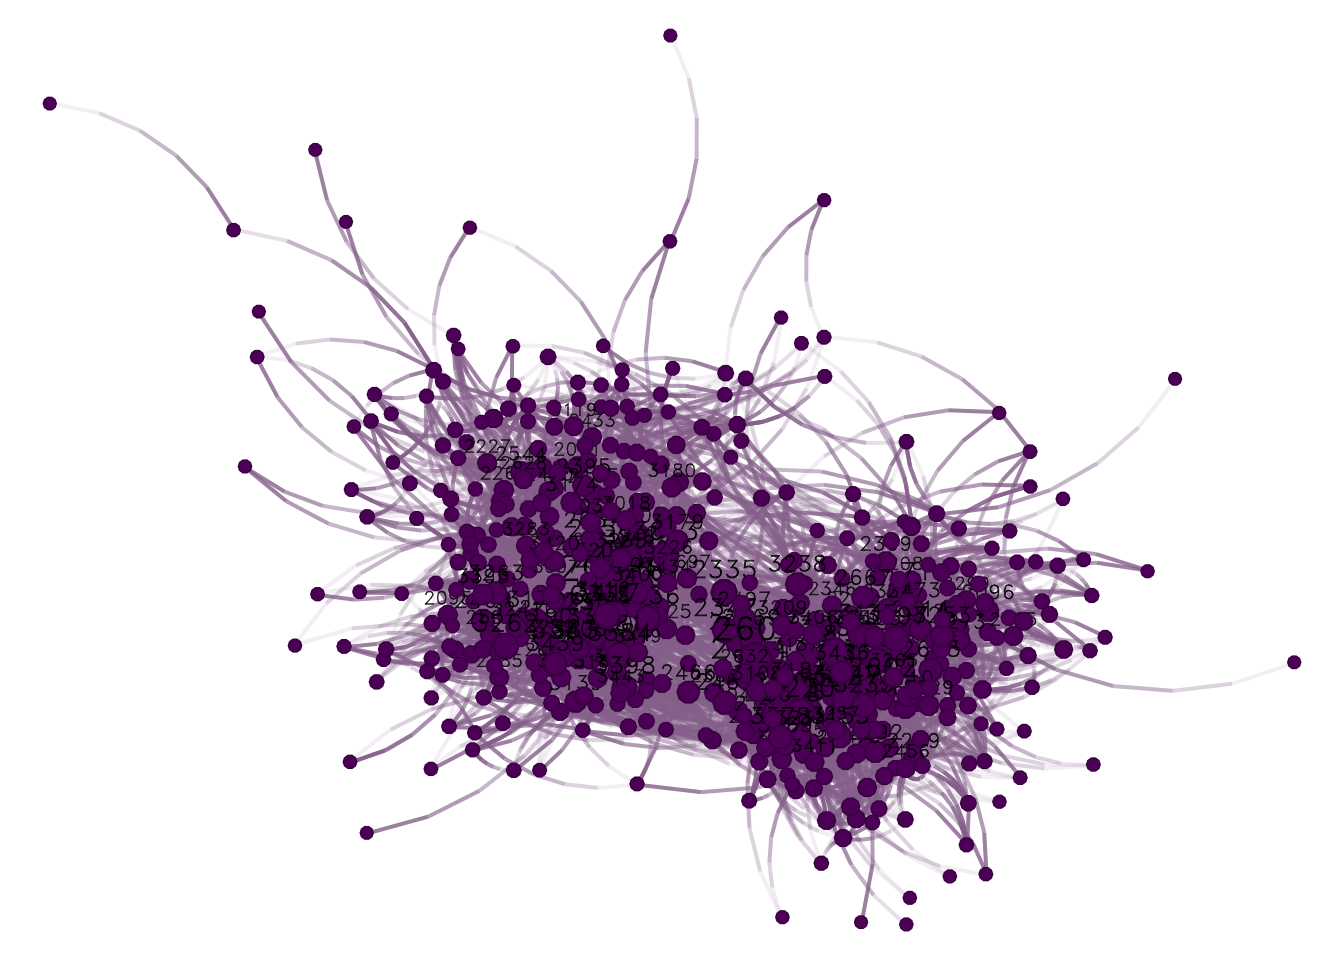
\includegraphics{paper_files/figure-pdf/plot_school1-1.pdf}

}

\end{figure}

\hypertarget{split-according-to-grade}{%
\paragraph{Split according to Grade}\label{split-according-to-grade}}

Here, we are taking the data set and coloring the nodes according to
grades. The 7th graders are in gray and the 8th graders are in red.

\begin{Shaded}
\begin{Highlighting}[]
\DocumentationTok{\#\# adjust \textquotesingle{}grade\textquotesingle{} to factor }
\FunctionTok{V}\NormalTok{(net\_with\_no\_isolates)}\SpecialCharTok{$}\NormalTok{grade }\OtherTok{\textless{}{-}}  \FunctionTok{as.factor}\NormalTok{(}\FunctionTok{V}\NormalTok{(net\_with\_no\_isolates)}\SpecialCharTok{$}\NormalTok{grade)  }

\CommentTok{\# plotting connections among grades \#\#\#\#}
\FunctionTok{set.seed}\NormalTok{(}\DecValTok{77}\NormalTok{)   }

\NormalTok{a\_colors }\OtherTok{\textless{}{-}} \FunctionTok{color\_nodes}\NormalTok{(net\_with\_no\_isolates,}\StringTok{"grade"}\NormalTok{, }\FunctionTok{c}\NormalTok{(}\StringTok{"gray40"}\NormalTok{,}\StringTok{"red3"}\NormalTok{))}
\FunctionTok{attr}\NormalTok{(a\_colors, }\StringTok{"map"}\NormalTok{)}
\end{Highlighting}
\end{Shaded}

\begin{verbatim}
        7         8 
"#666666" "#CD0000" 
\end{verbatim}

\begin{Shaded}
\begin{Highlighting}[]
\NormalTok{grades }\OtherTok{\textless{}{-}} \FunctionTok{nplot}\NormalTok{(}
\NormalTok{  net\_with\_no\_isolates,}
  \AttributeTok{vertex.color =} \FunctionTok{color\_nodes}\NormalTok{(net\_with\_no\_isolates, }\StringTok{"grade"}\NormalTok{, }\FunctionTok{c}\NormalTok{(}\StringTok{"gray40"}\NormalTok{,}\StringTok{"red3"}\NormalTok{)),}
  \AttributeTok{vertex.nsides =} \FunctionTok{ifelse}\NormalTok{(}\FunctionTok{V}\NormalTok{(net\_with\_no\_isolates)}\SpecialCharTok{$}\NormalTok{grade }\SpecialCharTok{==} \DecValTok{7}\NormalTok{, }\DecValTok{10}\NormalTok{, }\DecValTok{10}\NormalTok{),}
  \AttributeTok{vertex.size.range =} \FunctionTok{c}\NormalTok{(}\FloatTok{0.015}\NormalTok{, }\FloatTok{0.015}\NormalTok{),}
  \AttributeTok{edge.color =} \SpecialCharTok{\textasciitilde{}}\FunctionTok{ego}\NormalTok{(}\AttributeTok{alpha =} \DecValTok{1}\NormalTok{, }\AttributeTok{col =} \StringTok{"lightgray"}\NormalTok{) }\SpecialCharTok{+} \FunctionTok{alter}\NormalTok{(}\AttributeTok{alpha =} \FloatTok{0.25}\NormalTok{, }\AttributeTok{col =} \StringTok{"lightgray"}\NormalTok{),}
  \AttributeTok{vertex.label =} \ConstantTok{NULL}\NormalTok{,}
  \AttributeTok{edge.curvature =}\NormalTok{ pi}\SpecialCharTok{/}\DecValTok{6}\NormalTok{,}
  \AttributeTok{edge.line.breaks =} \DecValTok{10}  
\NormalTok{)  }

\CommentTok{\# add radial gradient fill }
\NormalTok{grades }\OtherTok{\textless{}{-}} \FunctionTok{set\_vertex\_gpar}\NormalTok{(grades, }
                          \AttributeTok{element =} \StringTok{"core"}\NormalTok{,}
                          \AttributeTok{fill =} \FunctionTok{lapply}\NormalTok{(}\FunctionTok{get\_vertex\_gpar}\NormalTok{(grades, }\StringTok{"frame"}\NormalTok{, }\StringTok{"col"}\NormalTok{)}\SpecialCharTok{$}\NormalTok{col, \textbackslash{}(i) \{}
                            \FunctionTok{radialGradient}\NormalTok{(}\FunctionTok{c}\NormalTok{(}\StringTok{"white"}\NormalTok{, i), }\AttributeTok{cx1=}\NormalTok{.}\DecValTok{8}\NormalTok{, }\AttributeTok{cy1=}\NormalTok{.}\DecValTok{8}\NormalTok{, }\AttributeTok{r1=}\DecValTok{0}\NormalTok{)}
\NormalTok{                          \}))}

\CommentTok{\# add legend to graph}
\NormalTok{grades\_general }\OtherTok{\textless{}{-}} \FunctionTok{nplot\_legend}\NormalTok{(}
\NormalTok{  grades,}
  \AttributeTok{labels =} \FunctionTok{c}\NormalTok{(}\StringTok{"7th"}\NormalTok{, }\StringTok{"8th"}\NormalTok{),}
  \AttributeTok{pch =} \FunctionTok{c}\NormalTok{(}\DecValTok{21}\NormalTok{,}\DecValTok{21}\NormalTok{),}
  \AttributeTok{gp =} \FunctionTok{gpar}\NormalTok{(}
    \AttributeTok{fill =} \FunctionTok{c}\NormalTok{(}\StringTok{"gray40"}\NormalTok{,}\StringTok{"red3"}\NormalTok{)),}
  \AttributeTok{packgrob.args =} \FunctionTok{list}\NormalTok{(}\AttributeTok{side =} \StringTok{"bottom"}\NormalTok{),}
  \AttributeTok{ncol =} \DecValTok{2}  
\NormalTok{)}


\NormalTok{grades\_general}
\FunctionTok{grid.text}\NormalTok{(}\StringTok{"Split According to Grade"}\NormalTok{, }\AttributeTok{x =}\NormalTok{ .}\DecValTok{2}\NormalTok{, }\AttributeTok{y =}\NormalTok{ .}\DecValTok{87}\NormalTok{, }\AttributeTok{just =} \StringTok{"bottom"}\NormalTok{) }
\end{Highlighting}
\end{Shaded}

\begin{figure}[H]

{\centering 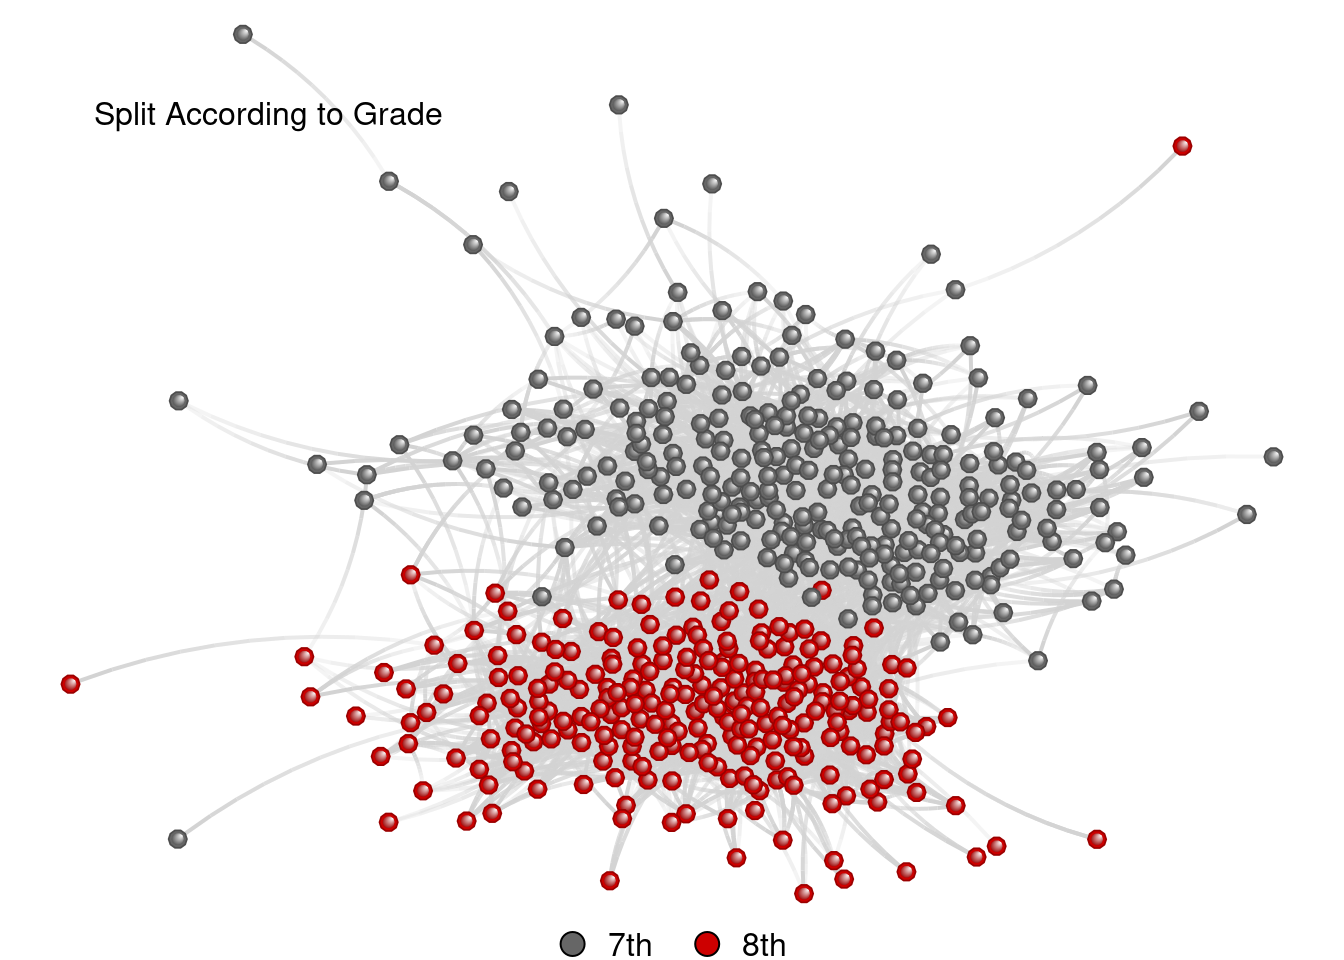
\includegraphics{paper_files/figure-pdf/grade-1.pdf}

}

\end{figure}

\hypertarget{split-according-to-gender}{%
\paragraph{Split according to Gender}\label{split-according-to-gender}}

Next, the data will be split according to gender, with male being yellow
and female being green. Also, the male points are circles, while the
female points are diamonds.

\begin{Shaded}
\begin{Highlighting}[]
\CommentTok{\# let\textquotesingle{}s get a graph for the gender data}
\FunctionTok{V}\NormalTok{(net\_with\_no\_isolates)}\SpecialCharTok{$}\NormalTok{gender }\OtherTok{\textless{}{-}}  \FunctionTok{as.factor}\NormalTok{(}\FunctionTok{V}\NormalTok{(net\_with\_no\_isolates)}\SpecialCharTok{$}\NormalTok{gender)}

\NormalTok{a\_colors }\OtherTok{\textless{}{-}} \FunctionTok{color\_nodes}\NormalTok{(net\_with\_no\_isolates,}\StringTok{"gender"}\NormalTok{, }\FunctionTok{c}\NormalTok{(}\StringTok{"lightgoldenrod2"}\NormalTok{,}\StringTok{"forestgreen"}\NormalTok{))}
\FunctionTok{attr}\NormalTok{(a\_colors, }\StringTok{"map"}\NormalTok{)}
\end{Highlighting}
\end{Shaded}

\begin{verbatim}
        0         1 
"#EEDC82" "#228B22" 
\end{verbatim}

\begin{Shaded}
\begin{Highlighting}[]
\DocumentationTok{\#\# plot}
\FunctionTok{set.seed}\NormalTok{(}\DecValTok{77}\NormalTok{)}
\NormalTok{gender }\OtherTok{\textless{}{-}} \FunctionTok{nplot}\NormalTok{(}
\NormalTok{  net\_with\_no\_isolates,}
  \AttributeTok{vertex.color =} \FunctionTok{color\_nodes}\NormalTok{(net\_with\_no\_isolates, }\StringTok{"gender"}\NormalTok{,}\FunctionTok{c}\NormalTok{(}\StringTok{"lightgoldenrod2"}\NormalTok{,}\StringTok{"forestgreen"}\NormalTok{)),}
  \AttributeTok{vertex.nsides =} \FunctionTok{ifelse}\NormalTok{(}\FunctionTok{V}\NormalTok{(net\_with\_no\_isolates)}\SpecialCharTok{$}\NormalTok{gender }\SpecialCharTok{==} \DecValTok{0}\NormalTok{, }\DecValTok{10}\NormalTok{, }\DecValTok{4}\NormalTok{),}
  \AttributeTok{vertex.size.range =} \FunctionTok{c}\NormalTok{(}\FloatTok{0.01}\NormalTok{, }\FloatTok{0.01}\NormalTok{),}
  \AttributeTok{edge.color =} \SpecialCharTok{\textasciitilde{}}\FunctionTok{ego}\NormalTok{(}\AttributeTok{alpha =} \FloatTok{0.33}\NormalTok{, }\AttributeTok{col =} \StringTok{"gray"}\NormalTok{) }\SpecialCharTok{+} \FunctionTok{alter}\NormalTok{(}\AttributeTok{alpha =} \FloatTok{0.33}\NormalTok{, }\AttributeTok{col =} \StringTok{"gray"}\NormalTok{),}
  \AttributeTok{vertex.label =} \ConstantTok{NULL}\NormalTok{,}
  \AttributeTok{edge.line.breaks =} \DecValTok{10}
\NormalTok{)}

\CommentTok{\# add legend to graph}
\FunctionTok{nplot\_legend}\NormalTok{(}
\NormalTok{  gender,}
  \AttributeTok{labels =} \FunctionTok{c}\NormalTok{(}\StringTok{"Male"}\NormalTok{, }\StringTok{"Female"}\NormalTok{),}
  \AttributeTok{pch =} \FunctionTok{c}\NormalTok{(}\DecValTok{21}\NormalTok{,}\DecValTok{23}\NormalTok{),}
  \AttributeTok{gp =} \FunctionTok{gpar}\NormalTok{(}
    \AttributeTok{fill =} \FunctionTok{c}\NormalTok{(}\StringTok{"lightgoldenrod2"}\NormalTok{,}\StringTok{"forestgreen"}\NormalTok{)),}
  \AttributeTok{packgrob.args =} \FunctionTok{list}\NormalTok{(}\AttributeTok{side =} \StringTok{"bottom"}\NormalTok{),}
  \AttributeTok{ncol =} \DecValTok{2}
\NormalTok{)}

\FunctionTok{grid.text}\NormalTok{(}\StringTok{"Split According to Gender"}\NormalTok{, }\AttributeTok{x =}\NormalTok{ .}\DecValTok{2}\NormalTok{, }\AttributeTok{y =}\NormalTok{ .}\DecValTok{87}\NormalTok{, }\AttributeTok{just =} \StringTok{"bottom"}\NormalTok{) }
\end{Highlighting}
\end{Shaded}

\begin{figure}[H]

{\centering 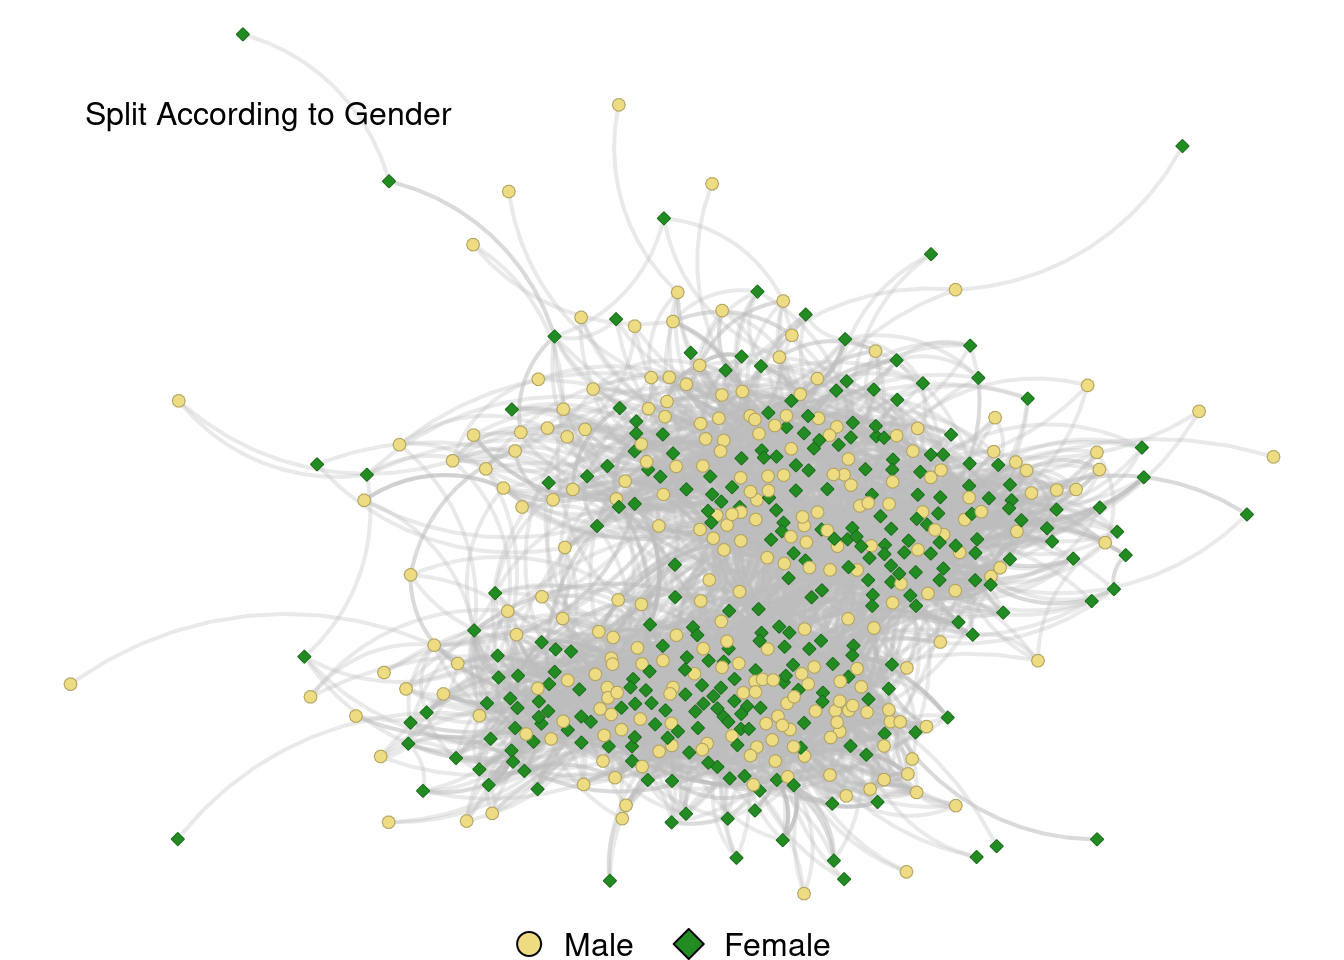
\includegraphics{paper_files/figure-pdf/gender-1.pdf}

}

\end{figure}

\hypertarget{split-according-to-lunch-period}{%
\paragraph{Split according to Lunch
Period}\label{split-according-to-lunch-period}}

Here is the data split according to the different lunch periods students
might be in.

\begin{Shaded}
\begin{Highlighting}[]
\CommentTok{\# now let\textquotesingle{}s do the same with lunch period }
\FunctionTok{V}\NormalTok{(net\_with\_no\_isolates)}\SpecialCharTok{$}\NormalTok{lunch }\OtherTok{\textless{}{-}}  \FunctionTok{as.factor}\NormalTok{(}\FunctionTok{V}\NormalTok{(net\_with\_no\_isolates)}\SpecialCharTok{$}\NormalTok{lunch)}

\NormalTok{a\_colors }\OtherTok{\textless{}{-}} \FunctionTok{color\_nodes}\NormalTok{(net\_with\_no\_isolates,}\StringTok{"lunch"}\NormalTok{, }\FunctionTok{c}\NormalTok{(}\StringTok{"purple"}\NormalTok{,}\StringTok{"palegreen"}\NormalTok{,}\StringTok{"steelblue"}\NormalTok{))}
\FunctionTok{attr}\NormalTok{(a\_colors, }\StringTok{"map"}\NormalTok{)}
\end{Highlighting}
\end{Shaded}

\begin{verbatim}
        1         2        99 
"#A020F0" "#98FB98" "#4682B4" 
\end{verbatim}

\begin{Shaded}
\begin{Highlighting}[]
\DocumentationTok{\#\# plot}
\FunctionTok{set.seed}\NormalTok{(}\DecValTok{77}\NormalTok{)}
\NormalTok{lunch }\OtherTok{\textless{}{-}} \FunctionTok{nplot}\NormalTok{(}
\NormalTok{  net\_with\_no\_isolates,}
  \AttributeTok{vertex.color =} \FunctionTok{color\_nodes}\NormalTok{(net\_with\_no\_isolates, }\StringTok{"lunch"}\NormalTok{,}\FunctionTok{c}\NormalTok{(}\StringTok{"purple"}\NormalTok{,}\StringTok{"palegreen"}\NormalTok{,}\StringTok{"steelblue"}\NormalTok{)),}
  \AttributeTok{vertex.nsides =} 
  \FunctionTok{ifelse}\NormalTok{(}\FunctionTok{V}\NormalTok{(net\_with\_no\_isolates)}\SpecialCharTok{$}\NormalTok{gender }\SpecialCharTok{==} \DecValTok{0}\NormalTok{, }\DecValTok{4}\NormalTok{,   }\CommentTok{\# First Lunch}
        \FunctionTok{ifelse}\NormalTok{(}\FunctionTok{V}\NormalTok{(net\_with\_no\_isolates)}\SpecialCharTok{$}\NormalTok{gender }\SpecialCharTok{==} \DecValTok{1}\NormalTok{, }\DecValTok{3}\NormalTok{,  }\CommentTok{\# Second Lunch }
               \DecValTok{10}\NormalTok{)),                                 }\CommentTok{\# Other}
  \AttributeTok{vertex.size.range =} \FunctionTok{c}\NormalTok{(}\FloatTok{0.01}\NormalTok{, }\FloatTok{0.01}\NormalTok{),}
  \AttributeTok{edge.color =} \SpecialCharTok{\textasciitilde{}}\FunctionTok{ego}\NormalTok{(}\AttributeTok{alpha =} \FloatTok{0.33}\NormalTok{, }\AttributeTok{col =} \StringTok{"gray"}\NormalTok{) }\SpecialCharTok{+} \FunctionTok{alter}\NormalTok{(}\AttributeTok{alpha =} \FloatTok{0.33}\NormalTok{, }\AttributeTok{col =} \StringTok{"gray"}\NormalTok{),}
  \AttributeTok{vertex.label =} \ConstantTok{NULL}\NormalTok{,}
  \AttributeTok{edge.line.breaks =} \DecValTok{10}
\NormalTok{)}

\CommentTok{\# add legend to graph}
\FunctionTok{nplot\_legend}\NormalTok{(}
\NormalTok{  lunch,}
  \AttributeTok{labels =} \FunctionTok{c}\NormalTok{(}\StringTok{"First"}\NormalTok{, }\StringTok{"Second"}\NormalTok{, }\StringTok{"Other"}\NormalTok{),}
  \AttributeTok{pch =} \FunctionTok{c}\NormalTok{(}\DecValTok{23}\NormalTok{,}\DecValTok{24}\NormalTok{,}\DecValTok{21}\NormalTok{),}
  \AttributeTok{gp =} \FunctionTok{gpar}\NormalTok{(}
    \AttributeTok{fill =} \FunctionTok{c}\NormalTok{(}\StringTok{"purple"}\NormalTok{,}\StringTok{"palegreen"}\NormalTok{,}\StringTok{"steelblue"}\NormalTok{)),}
  \AttributeTok{packgrob.args =} \FunctionTok{list}\NormalTok{(}\AttributeTok{side =} \StringTok{"bottom"}\NormalTok{),}
  \AttributeTok{ncol =} \DecValTok{3}
\NormalTok{)}

\FunctionTok{grid.text}\NormalTok{(}\StringTok{"Split According to Lunch Period"}\NormalTok{, }\AttributeTok{x =}\NormalTok{ .}\DecValTok{2}\NormalTok{, }\AttributeTok{y =}\NormalTok{ .}\DecValTok{87}\NormalTok{, }\AttributeTok{just =} \StringTok{"bottom"}\NormalTok{) }
\end{Highlighting}
\end{Shaded}

\begin{figure}[H]

{\centering 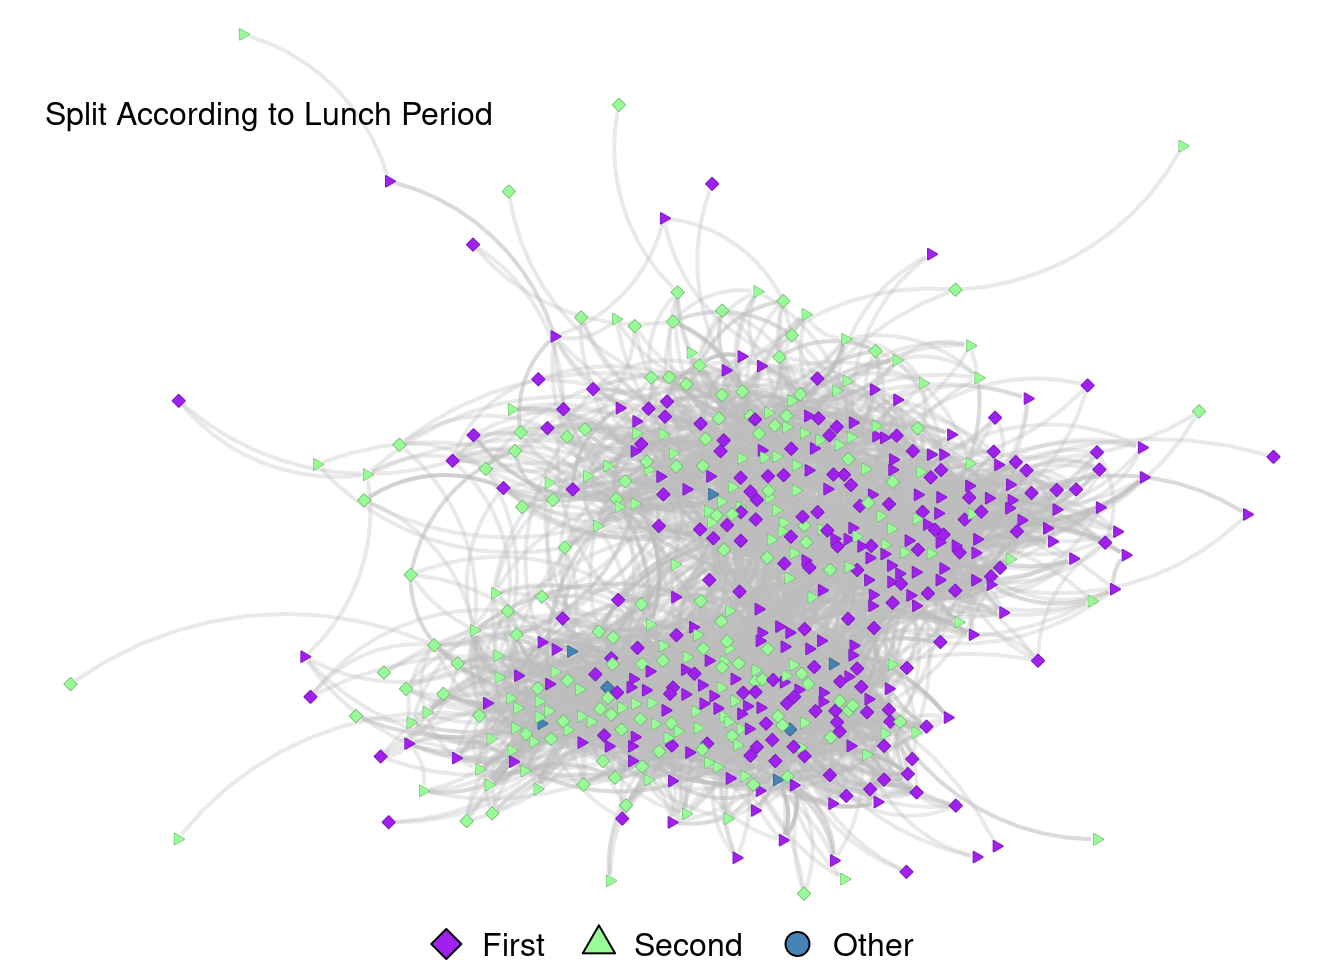
\includegraphics{paper_files/figure-pdf/lunch-1.pdf}

}

\end{figure}

\hypertarget{changing-lines-to-dashes}{%
\paragraph{Changing Lines to Dashes}\label{changing-lines-to-dashes}}

One of the perks of \texttt{netplot} is the ability to be fully
customizable, right out of the box. First, here is an example of the
same dataset, but the edges are dashed instead of full and straight
instead of curved.

\begin{Shaded}
\begin{Highlighting}[]
\FunctionTok{set.seed}\NormalTok{(}\DecValTok{77}\NormalTok{)}

\NormalTok{grades }\OtherTok{\textless{}{-}} \FunctionTok{nplot}\NormalTok{(}
\NormalTok{  net\_with\_no\_isolates,}
  \AttributeTok{bg.col =} \StringTok{"\#F5F5F5"}\NormalTok{,}
  \AttributeTok{vertex.color =} \FunctionTok{color\_nodes}\NormalTok{(net\_with\_no\_isolates, }\StringTok{"grade"}\NormalTok{, }\FunctionTok{c}\NormalTok{(}\StringTok{"red"}\NormalTok{,}\StringTok{"blue"}\NormalTok{)),}
  \AttributeTok{vertex.size.range =} \FunctionTok{c}\NormalTok{(}\FloatTok{0.02}\NormalTok{, }\FloatTok{0.02}\NormalTok{),}
  \AttributeTok{edge.color =} \SpecialCharTok{\textasciitilde{}}\FunctionTok{ego}\NormalTok{(}\AttributeTok{alpha =}\NormalTok{ .}\DecValTok{15}\NormalTok{, }\AttributeTok{col =} \StringTok{"black"}\NormalTok{) }\SpecialCharTok{+} \FunctionTok{alter}\NormalTok{(}\AttributeTok{alpha =}\NormalTok{ .}\DecValTok{15}\NormalTok{, }\AttributeTok{col =} \StringTok{"black"}\NormalTok{),}
  \AttributeTok{vertex.label =} \ConstantTok{NULL}\NormalTok{,}
  \AttributeTok{edge.width.range =} \FunctionTok{c}\NormalTok{(}\DecValTok{2}\NormalTok{,}\DecValTok{2}\NormalTok{),}
  \AttributeTok{edge.line.lty =} \DecValTok{6}\NormalTok{,}
  \AttributeTok{edge.line.breaks =} \DecValTok{1}  
\NormalTok{)  }



\CommentTok{\# add legend to graph}
\NormalTok{grades\_dashed }\OtherTok{\textless{}{-}} \FunctionTok{nplot\_legend}\NormalTok{(}
\NormalTok{  grades,}
  \AttributeTok{labels =} \FunctionTok{c}\NormalTok{(}\StringTok{"7th"}\NormalTok{, }\StringTok{"8th"}\NormalTok{),}
  \AttributeTok{pch =} \FunctionTok{c}\NormalTok{(}\DecValTok{21}\NormalTok{,}\DecValTok{21}\NormalTok{),}
  \AttributeTok{gp =} \FunctionTok{gpar}\NormalTok{(}
    \AttributeTok{fill =} \FunctionTok{c}\NormalTok{(}\StringTok{"red"}\NormalTok{,}\StringTok{"blue"}\NormalTok{)),}
  \AttributeTok{packgrob.args =} \FunctionTok{list}\NormalTok{(}\AttributeTok{side =} \StringTok{"bottom"}\NormalTok{),}
  \AttributeTok{ncol =} \DecValTok{2}  
\NormalTok{)}

\NormalTok{grades\_dashed}
\end{Highlighting}
\end{Shaded}

\begin{figure}[H]

{\centering 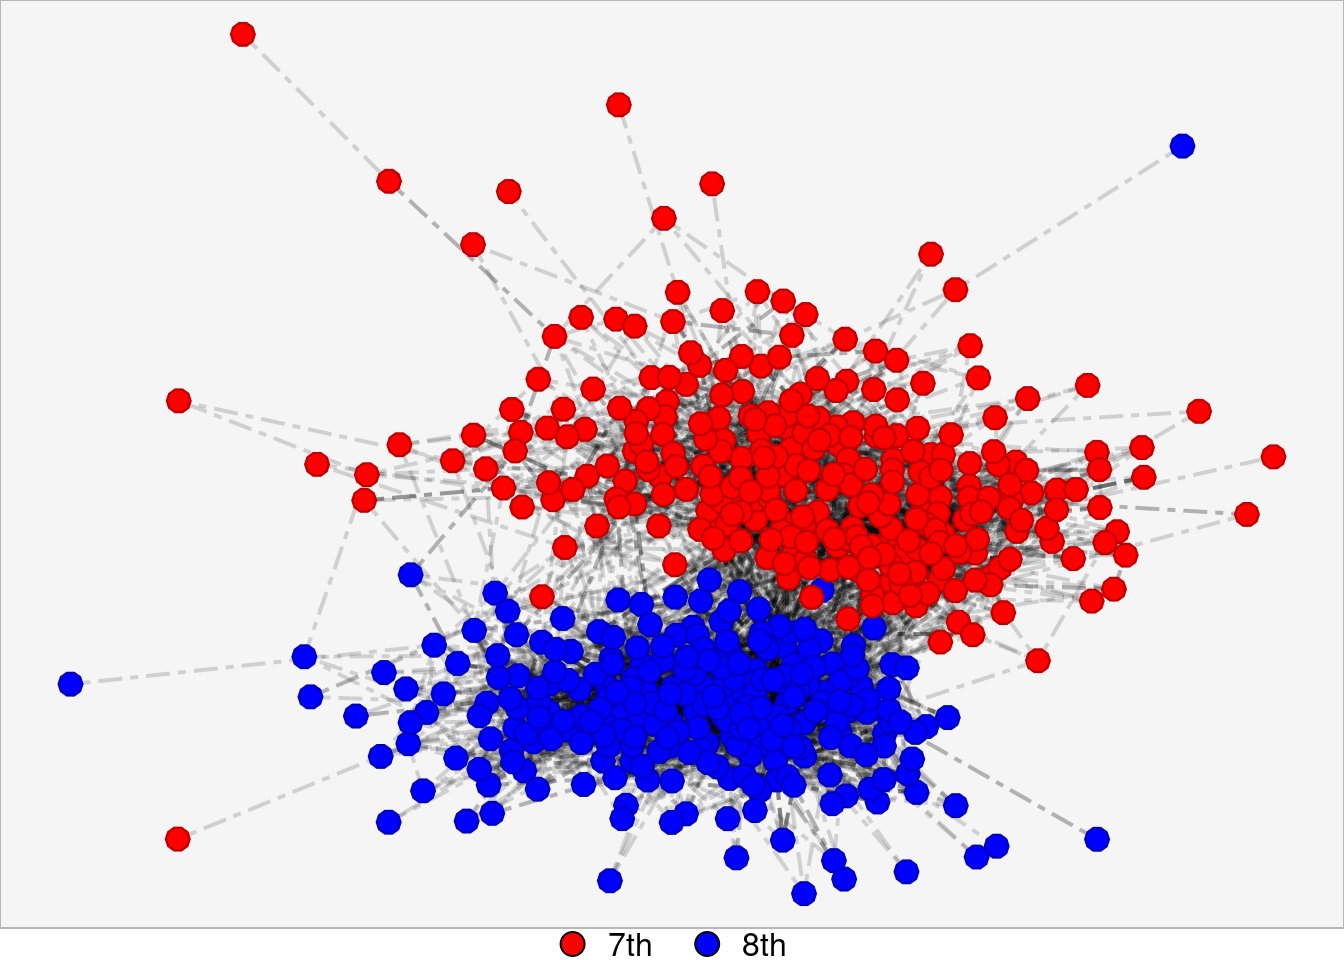
\includegraphics{paper_files/figure-pdf/dashes-1.pdf}

}

\end{figure}

\hypertarget{colored-edges-and-skipped-vertices}{%
\subsubsection{Colored Edges and Skipped
Vertices}\label{colored-edges-and-skipped-vertices}}

This selection shows how to skip vertices and add colors to the edges.

\begin{Shaded}
\begin{Highlighting}[]
\FunctionTok{set.seed}\NormalTok{(}\DecValTok{77}\NormalTok{)   }

\NormalTok{grades }\OtherTok{\textless{}{-}} \FunctionTok{nplot}\NormalTok{(}
\NormalTok{  net\_with\_no\_isolates,}
  \AttributeTok{bg.col =} \StringTok{"\#F5F5F5"}\NormalTok{,}
  \AttributeTok{vertex.color =} \FunctionTok{color\_nodes}\NormalTok{(net\_with\_no\_isolates, }\StringTok{"grade"}\NormalTok{, }\FunctionTok{c}\NormalTok{(}\StringTok{"red"}\NormalTok{,}\StringTok{"blue"}\NormalTok{)),}
  \AttributeTok{vertex.nsides =} \FunctionTok{ifelse}\NormalTok{(}\FunctionTok{V}\NormalTok{(net\_with\_no\_isolates)}\SpecialCharTok{$}\NormalTok{grade }\SpecialCharTok{==} \DecValTok{7}\NormalTok{, }\DecValTok{10}\NormalTok{, }\DecValTok{4}\NormalTok{),}
  \AttributeTok{vertex.size.range =} \FunctionTok{c}\NormalTok{(}\FloatTok{0.0001}\NormalTok{, }\FloatTok{0.0001}\NormalTok{),}
  \AttributeTok{edge.color =} \SpecialCharTok{\textasciitilde{}}\FunctionTok{ego}\NormalTok{(}\AttributeTok{alpha =} \FloatTok{0.33}\NormalTok{) }\SpecialCharTok{+} \FunctionTok{alter}\NormalTok{(}\AttributeTok{alpha =} \FloatTok{0.33}\NormalTok{),}
  \AttributeTok{vertex.label =} \ConstantTok{NULL}\NormalTok{,}
  \AttributeTok{edge.width.range =} \FunctionTok{c}\NormalTok{(}\DecValTok{2}\NormalTok{,}\DecValTok{2}\NormalTok{),}
  \AttributeTok{edge.line.breaks =} \DecValTok{10}
\NormalTok{  )  }

\CommentTok{\# add legend to graph}
\NormalTok{grades\_edge\_colored }\OtherTok{\textless{}{-}} \FunctionTok{nplot\_legend}\NormalTok{(}
\NormalTok{  grades,}
  \AttributeTok{labels =} \FunctionTok{c}\NormalTok{(}\StringTok{"7th"}\NormalTok{, }\StringTok{"8th"}\NormalTok{),}
  \AttributeTok{pch =} \FunctionTok{c}\NormalTok{(}\DecValTok{21}\NormalTok{,}\DecValTok{21}\NormalTok{),}
  \AttributeTok{gp =} \FunctionTok{gpar}\NormalTok{(}
    \AttributeTok{fill =} \FunctionTok{c}\NormalTok{(}\StringTok{"red"}\NormalTok{,}\StringTok{"blue"}\NormalTok{)),}
  \AttributeTok{packgrob.args =} \FunctionTok{list}\NormalTok{(}\AttributeTok{side =} \StringTok{"bottom"}\NormalTok{),}
  \AttributeTok{ncol =} \DecValTok{2}
\NormalTok{  )}

\NormalTok{grades\_edge\_colored}
\end{Highlighting}
\end{Shaded}

\begin{figure}[H]

{\centering 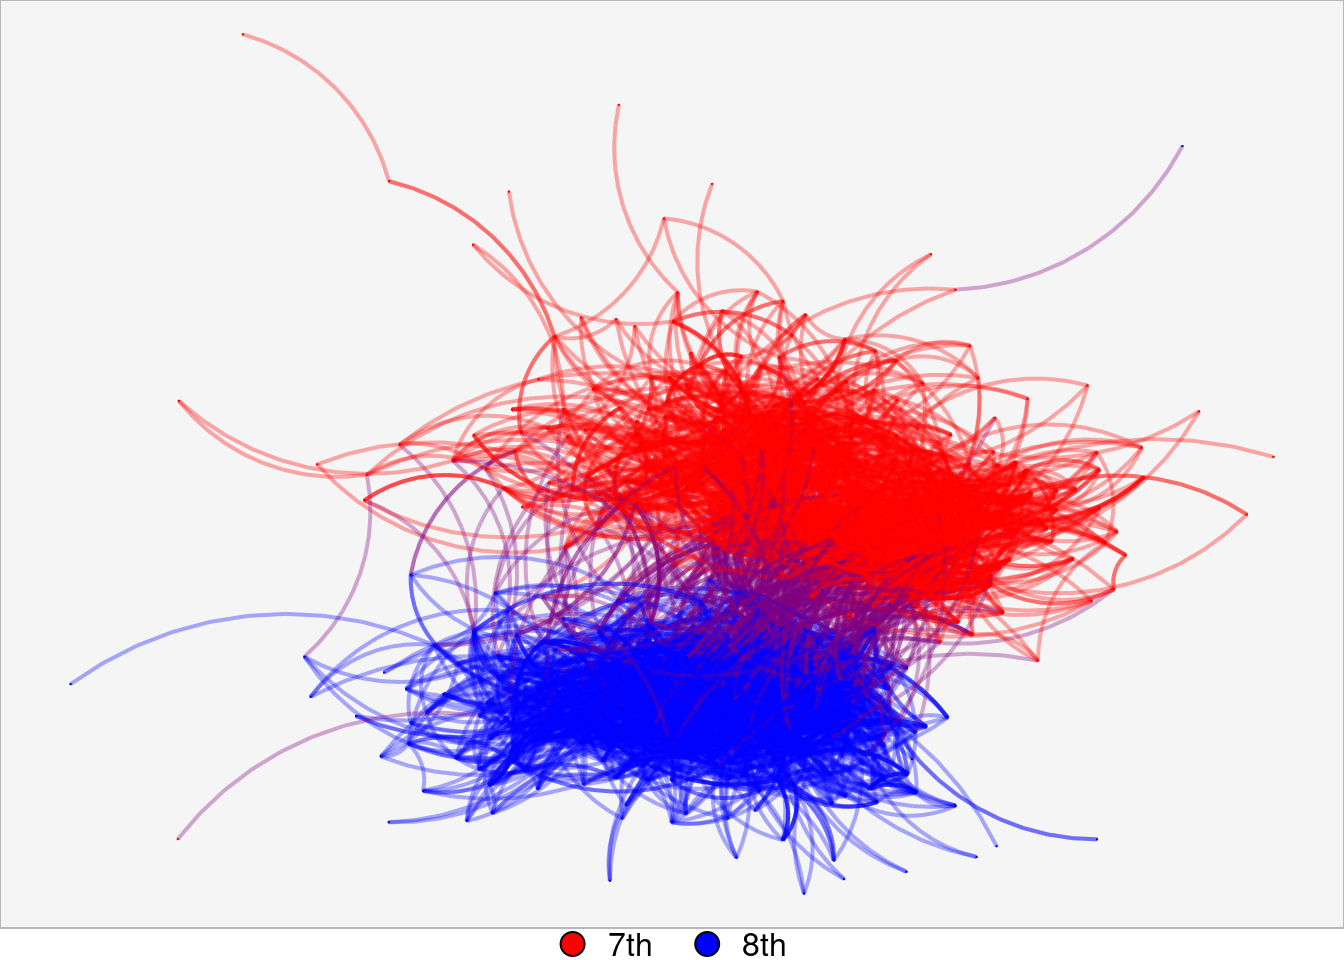
\includegraphics{paper_files/figure-pdf/skipped-1.pdf}

}

\end{figure}

\hypertarget{changing-background-color}{%
\subsubsection{Changing Background
Color}\label{changing-background-color}}

We can also add a background to the plot, including a gradient.

\begin{Shaded}
\begin{Highlighting}[]
\FunctionTok{set.seed}\NormalTok{(}\DecValTok{77}\NormalTok{)   }

\NormalTok{grades }\OtherTok{\textless{}{-}} \FunctionTok{nplot}\NormalTok{(}
\NormalTok{  net\_with\_no\_isolates,}
  \AttributeTok{bg.col =} \FunctionTok{linearGradient}\NormalTok{(}\FunctionTok{c}\NormalTok{(}\StringTok{"lightpink"}\NormalTok{, }\StringTok{"lightskyblue"}\NormalTok{)),}
  \AttributeTok{vertex.color =} \FunctionTok{color\_nodes}\NormalTok{(net\_with\_no\_isolates, }\StringTok{"grade"}\NormalTok{, }\FunctionTok{c}\NormalTok{(}\StringTok{"red"}\NormalTok{,}\StringTok{"blue"}\NormalTok{)),}
  \AttributeTok{vertex.nsides =} \FunctionTok{ifelse}\NormalTok{(}\FunctionTok{V}\NormalTok{(net\_with\_no\_isolates)}\SpecialCharTok{$}\NormalTok{grade }\SpecialCharTok{==} \DecValTok{7}\NormalTok{, }\DecValTok{10}\NormalTok{, }\DecValTok{4}\NormalTok{),}
  \AttributeTok{vertex.size.range =} \FunctionTok{c}\NormalTok{(}\FloatTok{0.01}\NormalTok{, }\FloatTok{0.01}\NormalTok{),}
  \AttributeTok{edge.color =} \SpecialCharTok{\textasciitilde{}}\FunctionTok{ego}\NormalTok{(}\AttributeTok{alpha =} \FloatTok{0.15}\NormalTok{, }\AttributeTok{col =} \StringTok{"black"}\NormalTok{) }\SpecialCharTok{+} \FunctionTok{alter}\NormalTok{(}\AttributeTok{alpha =} \FloatTok{0.15}\NormalTok{, }\AttributeTok{col =} \StringTok{"black"}\NormalTok{),}
  \AttributeTok{vertex.label =} \ConstantTok{NULL}\NormalTok{,}
  \AttributeTok{edge.line.breaks =} \DecValTok{10}  
\NormalTok{)  }

\CommentTok{\# add legend to graph}
\NormalTok{grades\_background }\OtherTok{\textless{}{-}} \FunctionTok{nplot\_legend}\NormalTok{(}
\NormalTok{  grades,}
  \AttributeTok{labels =} \FunctionTok{c}\NormalTok{(}\StringTok{"7th"}\NormalTok{, }\StringTok{"8th"}\NormalTok{),}
  \AttributeTok{pch =} \FunctionTok{c}\NormalTok{(}\DecValTok{21}\NormalTok{,}\DecValTok{23}\NormalTok{),}
  \AttributeTok{gp =} \FunctionTok{gpar}\NormalTok{(}
    \AttributeTok{fill =} \FunctionTok{c}\NormalTok{(}\StringTok{"red"}\NormalTok{,}\StringTok{"blue"}\NormalTok{)),}
  \AttributeTok{packgrob.args =} \FunctionTok{list}\NormalTok{(}\AttributeTok{side =} \StringTok{"bottom"}\NormalTok{),}
  \AttributeTok{ncol =} \DecValTok{2}  
\NormalTok{)}

\NormalTok{grades\_background}
\end{Highlighting}
\end{Shaded}

\begin{figure}[H]

{\centering 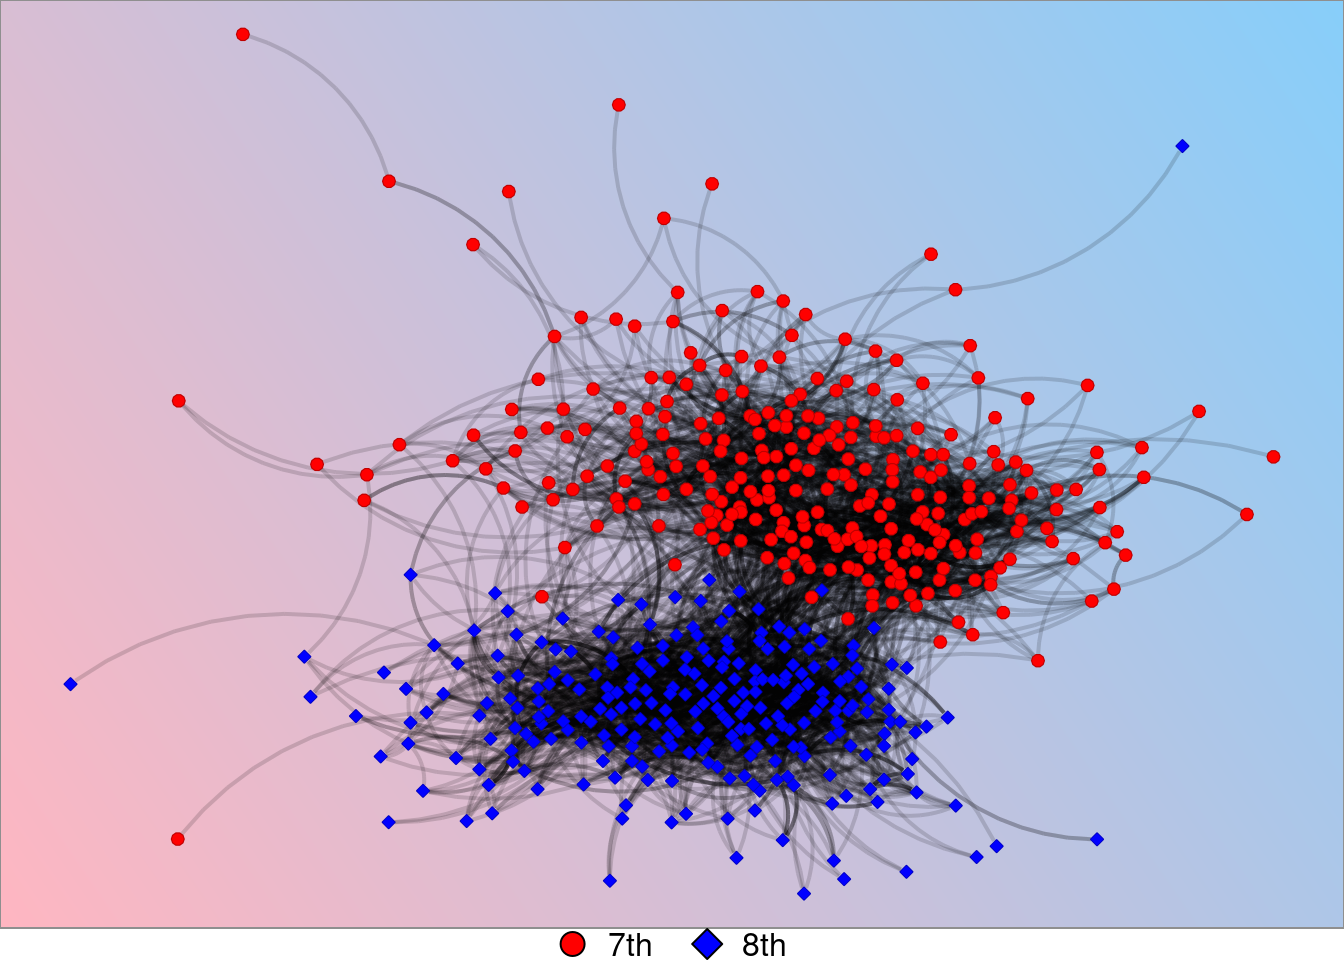
\includegraphics{paper_files/figure-pdf/background-1.pdf}

}

\end{figure}

\hypertarget{different-colors}{%
\subsubsection{Different Colors}\label{different-colors}}

We can also change vertex colors and edges to straight lines.

\begin{Shaded}
\begin{Highlighting}[]
\FunctionTok{set.seed}\NormalTok{(}\DecValTok{77}\NormalTok{)}

\NormalTok{grades }\OtherTok{\textless{}{-}} \FunctionTok{nplot}\NormalTok{(}
\NormalTok{  net\_with\_no\_isolates,}
  \AttributeTok{bg.col =} \StringTok{"\#F5F5F5"}\NormalTok{,}
  \AttributeTok{vertex.color =} \FunctionTok{color\_nodes}\NormalTok{(net\_with\_no\_isolates, }\StringTok{"grade"}\NormalTok{, }\FunctionTok{c}\NormalTok{(}\StringTok{"\#FFDB58"}\NormalTok{,}\StringTok{"\#708090"}\NormalTok{)),}
  \AttributeTok{vertex.nsides =} \FunctionTok{ifelse}\NormalTok{(}\FunctionTok{V}\NormalTok{(net\_with\_no\_isolates)}\SpecialCharTok{$}\NormalTok{grade }\SpecialCharTok{==} \DecValTok{7}\NormalTok{, }\DecValTok{10}\NormalTok{, }\DecValTok{4}\NormalTok{),}
  \AttributeTok{vertex.size.range =} \FunctionTok{c}\NormalTok{(}\FloatTok{0.02}\NormalTok{, }\FloatTok{0.02}\NormalTok{),}
  \AttributeTok{edge.color =} \SpecialCharTok{\textasciitilde{}}\FunctionTok{ego}\NormalTok{(}\AttributeTok{alpha =}\NormalTok{ .}\DecValTok{15}\NormalTok{, }\AttributeTok{col =} \StringTok{"black"}\NormalTok{) }\SpecialCharTok{+} \FunctionTok{alter}\NormalTok{(}\AttributeTok{alpha =}\NormalTok{ .}\DecValTok{15}\NormalTok{, }\AttributeTok{col =} \StringTok{"black"}\NormalTok{),}
  \AttributeTok{vertex.label =} \ConstantTok{NULL}\NormalTok{,}
  \AttributeTok{edge.width.range =} \FunctionTok{c}\NormalTok{(}\DecValTok{2}\NormalTok{,}\DecValTok{2}\NormalTok{),}
  \AttributeTok{edge.line.breaks =} \DecValTok{1}
\NormalTok{)}

\CommentTok{\# add legend to graph}
\NormalTok{grades\_different\_color }\OtherTok{\textless{}{-}} \FunctionTok{nplot\_legend}\NormalTok{(}
\NormalTok{  grades,}
  \AttributeTok{labels =} \FunctionTok{c}\NormalTok{(}\StringTok{"7th"}\NormalTok{, }\StringTok{"8th"}\NormalTok{),}
  \AttributeTok{pch =} \FunctionTok{c}\NormalTok{(}\DecValTok{21}\NormalTok{,}\DecValTok{23}\NormalTok{),}
  \AttributeTok{gp =} \FunctionTok{gpar}\NormalTok{(}
    \AttributeTok{fill =} \FunctionTok{c}\NormalTok{(}\StringTok{"\#FFDB58"}\NormalTok{,}\StringTok{"\#708090"}\NormalTok{)),}
  \AttributeTok{packgrob.args =} \FunctionTok{list}\NormalTok{(}\AttributeTok{side =} \StringTok{"bottom"}\NormalTok{),}
  \AttributeTok{ncol =} \DecValTok{2}  
\NormalTok{)}

\NormalTok{grades\_different\_color}
\end{Highlighting}
\end{Shaded}

\begin{figure}[H]

{\centering 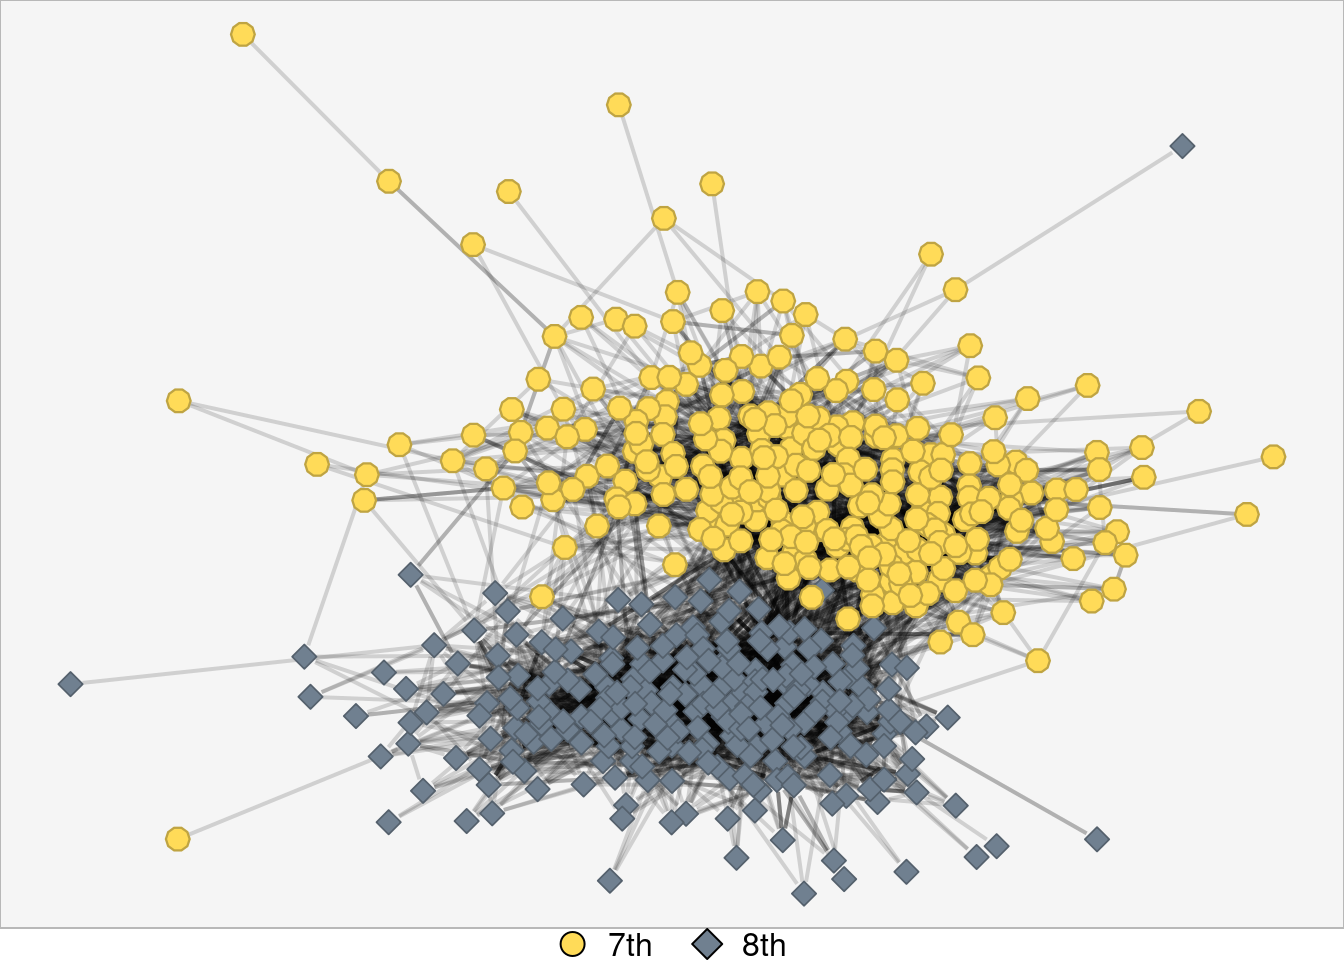
\includegraphics{paper_files/figure-pdf/colors-1.pdf}

}

\end{figure}

\hypertarget{example-2-ltcf-data}{%
\subsubsection{Example 2: LTCF data}\label{example-2-ltcf-data}}



\end{document}
